\documentclass{beamer}

\usepackage{Haust2017glærur}

\title{Tölvunarfræði 1a}
\subtitle{Vika 8, fyrri fyrirlestur}

\begin{document}

\begin{frame}
\titlepage
\end{frame}

\section{Inngangur}

\begin{frame}{Í síðasta þætti\ldots}
Meira um strengi
\end{frame}

\section{Miðmisserispróf}

\begin{frame}{Miðmisserispróf}
\pause
    \begin{itemize}
        \item 63 nemendur af 81 ($\approx$77\%) tóku prófið 
        \begin{itemize}
            \item 83\% árið 2016
            \item 79\% árið 2015
            \item 69\% árið 2014 
        \end{itemize} \pause
        \item Meðaleinkunn var $\approx$4.67 \pause
        \begin{itemize}
            \item 6.61 árið 2016
            \item 7.19 árið 2015
            \item 5.51 árið 2014
        \end{itemize}
    \end{itemize}
\end{frame}

\begin{frame}{Einkunnadreifingin}
\begin{center}
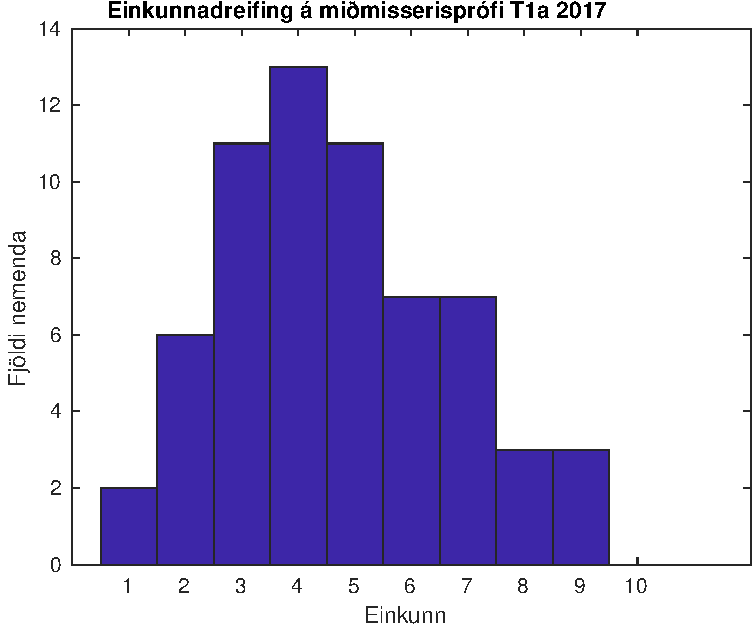
\includegraphics[width=0.8\textwidth]{midmisserisprof2017}
\end{center}
\end{frame}

\section{Miðmisseriskönnun}

\begin{frame}{Miðmisseriskönnun}
\begin{center}
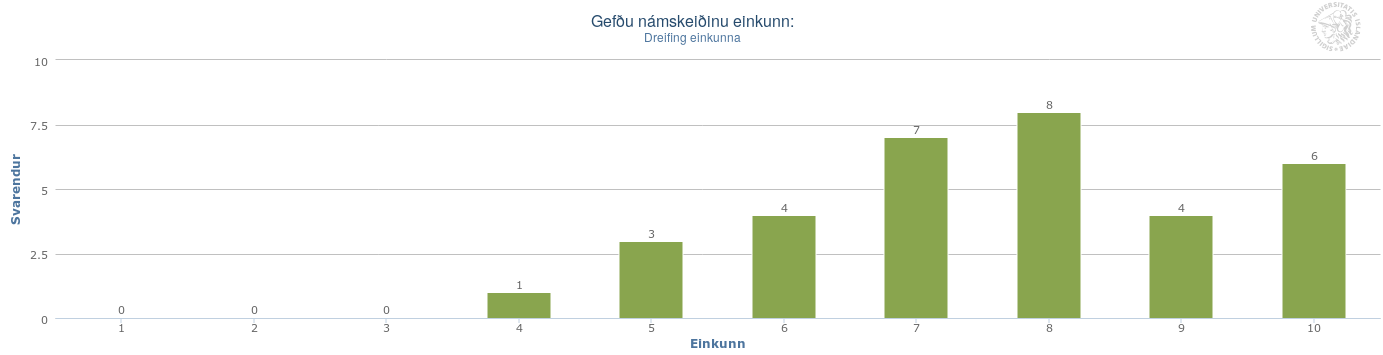
\includegraphics[width=\textwidth]{Dreifing2017}
\end{center}
Meðaleinkunn námskeiðsins var 7.64 (Meðaleinkunn IVT 7.8). 33/81 ($\approx$41\%) tóku þátt.
\end{frame}

\begin{frame}{Almenn ánægja}
    \begin{itemize}
        \item Fleiri jákvæðar en neikvæðar athugasemdir bárust um
        \begin{itemize}[<+->]
            \item Skipulag
            \item Alla kennarana
            \item Skilaverkefni
            \item Glærur
        \end{itemize}
    \end{itemize}
\end{frame}

\begin{frame}{Endurteknar athugasemdir}
    \begin{itemize}
        \item Örfáar athugasemdir bárust oftar en einu sinni
        \begin{itemize}
            \item Nemendur týndir í skilaverkefnum
            \item Vantar fleiri/hnitmiðaðri sýnidæmi í fyrirlestrum
            \item Fyrirlestrar/dæmatímar gagnslausir fyrir lengra komna
            \item Gert ráð fyrir forritunarþekkingu í upphafi
            \item Vantar stoðtíma
        \end{itemize}
    \end{itemize}
\end{frame}

\begin{frame}{Aðgerðir}
    \begin{itemize}
        \item Stoðtíminn á föstudögum verður fastur liður
        \item Leitast við að eyða meiri tíma með Matlab á skjánum í fyrirlestrum
        \item \emph{Fleiri uppástungur þegnar!}
    \end{itemize}
\end{frame}

\section{Gagnagrindur}

\begin{frame}{Gagnagrindur}
\begin{itemize}
 \item Gagnagrind (e. \emph{data structure}) er skilgreind aðferð við að geyma og skipuleggja gögn í minni tölvunnar þannig að hægt sé að vinna með þau á skilvirkan hátt
 \begin{itemize}
  \item Sumar gagnagrindur henta vel fyrir leit í gögnum
  \item Aðrar henta vel til að setja inn ný gögn
 \end{itemize}
 \item Val á gagnagrind getur skipt miklu máli
\end{itemize}
\end{frame}

\begin{frame}{Gagnagrindur í Matlab}
\begin{itemize}
 \item Höfum séð vigra og fylki
 \begin{itemize}
  \item Vigrar og fylki hafa ákveðið skipulag
  \begin{itemize}
   \item Gögnin í vigrum eru í númeruðum sætum, frá 1 til $n$
   \item Vigrar eru geymdir í samfelldu minnisplássi, svo það er auðvelt að ná í gildið í $k$-ta sætinu
\begin{center}
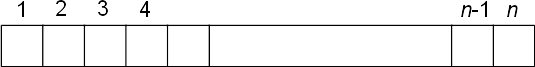
\includegraphics[width=0.6\textwidth]{Pics/vector-index}
\end{center}
   \end{itemize}
  \item Vigrar og fylki eru oftast góð gagnagrind fyrir einsleit gögn, sérstaklega þegar stærðin er þekkt fyrirfram
  \begin{itemize}
   \item Ef $v$ inniheldur \texttt{double} tölur, þá er $v(i)$ $8i$ bætum frá ``$v(0)$''
  \end{itemize}
 \end{itemize}
\end{itemize}
\end{frame}

\begin{frame}{Bendar}
    \begin{itemize}
        \item Bendir (e. \emph{pointers}) er breyta eða minnishólf sem inniheldur upplýsingar um staðsetningu annars minnishólfs
        \item Eru á bak við tjöldin í Matlab, mjög sýnilegir í forritunarmálinu C og ættingjum þess
        \item Hægt að nota benda til að halda utan um gögn í sundurlægum minnissvæðum
    \end{itemize}
\end{frame}

\begin{frame}{Dæmi um gagnagrind}
Eintengdur listi
\begin{center}
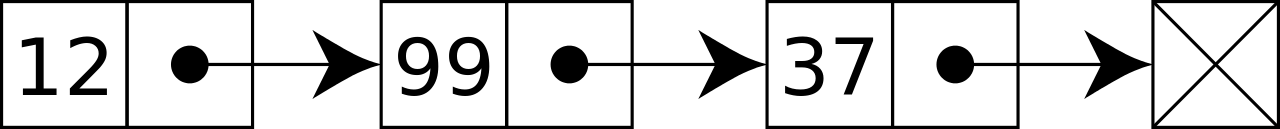
\includegraphics[width=\textwidth]{Pics/singly-linked-list}
\end{center}
\end{frame}

\begin{frame}{Dæmi um gagnagrind}
\vspace{\baselineskip}
Tré
\begin{center}
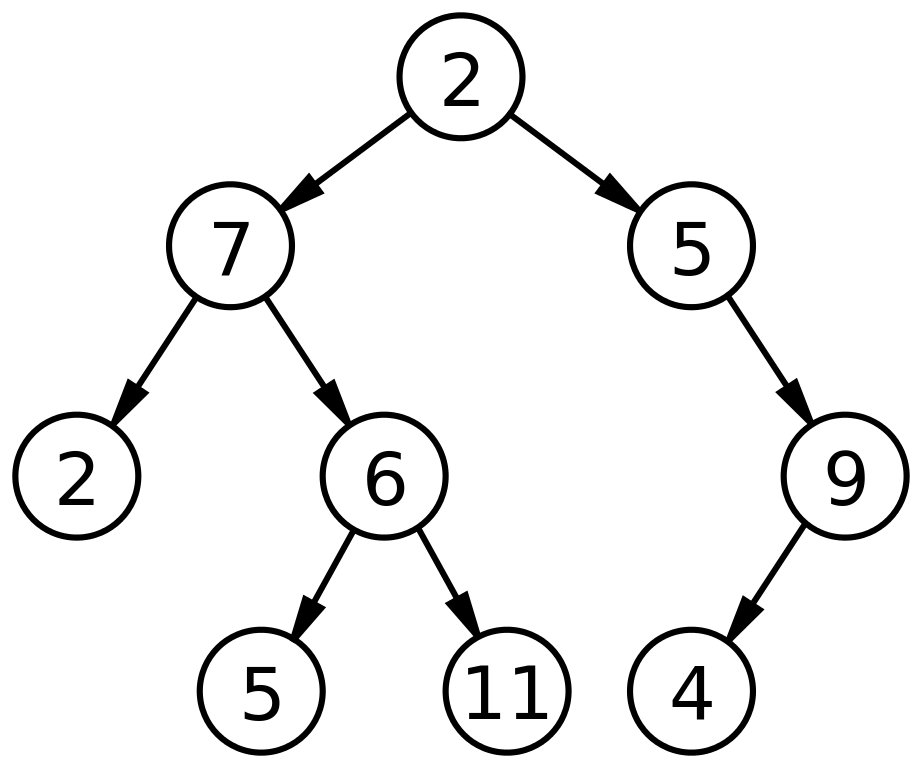
\includegraphics[width=0.6\textwidth]{Pics/tree}
\end{center}
\end{frame}

\begin{frame}{Dæmi um gagnagrind}
Hakkatafla
\begin{center}
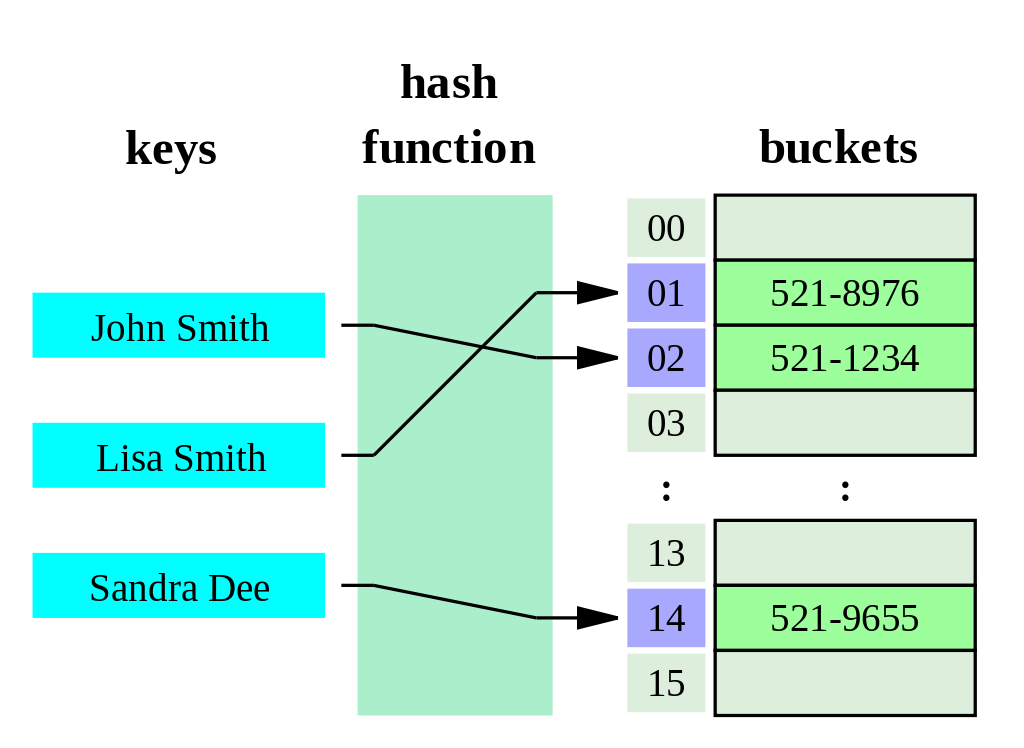
\includegraphics[width=0.6\textwidth]{Pics/hash-table}
\end{center}
\end{frame}

\section{Hólfafylki (8.1)}

\begin{frame}{Hólfafylki og hólfavigrar}
\begin{itemize}
 \item Hingað til höfum við lent í vandræðum við að geyma gögn sem ekki eru öll ``eins'' í einhverjum skilningi
 \begin{itemize}
  \item Nýlegasta dæmið: Mislangir strengir
 \end{itemize}
 \item Til að geyma safn af gögnum sem ekki eru öll ``eins'' í Matlab má nota nýja gagnagerð, svokallað hólfafylki (e. \emph{cell array})
 \item Hólfafylki komast fram hjá hefðbundnum minnissvæðatakmörkunum með því að geyma benda á önnur minnissvæði
\end{itemize}
\end{frame}

\begin{frame}[fragile]{Hólfafylki - dæmi}
Búa má til hólfafylki/hólfavigra með því að umlykja gögnin sem geyma skal með slaufusvigum:

\begin{minted}[frame=lines]{matlab}
>> cells = {'a', 'ab', 'abc', 1}
cells = 
    'a'    'ab'    'abc'    [1]
>> whos cells
  Name       Size            Bytes  Class    Attributes
  cells      1x4               468  cell
\end{minted}
\end{frame}

\begin{frame}[fragile]{Hólfafylki - dæmi}
Fyrri skipunin býr til $1\times 4$ hólfavigur, sú seinni $2 \times 2$ hólfafylki
\begin{minted}[frame=lines]{matlab}
>> ca = {23, 'a', 1:2:9, 'hello'} 
ca = 
   [23]   'a'   [1x5 double]   'hello'

>> cm = {23, 'a'; 1:2:9, 'hello'}
cm = 
    [        23]    'a'    
    [1x5 double]    'hello'
\end{minted}
\end{frame}

\begin{frame}[fragile]{Innihald hólfa}
\begin{columns}
\column{0.5\textwidth}
\begin{itemize}
 \item Hvert hólf í hólfavigri inniheldur einhverja tegund af Matlab vigri/fylki
 \item Getum líka forúthlutað hólfavigri með fallinu \texttt{cell}:
\end{itemize}
\column{0.5\textwidth}
\begin{minted}[frame=lines]{matlab}
>> cm1 = cell(2,2)
cm1 = 
    []    []
    []    []
\end{minted}
\end{columns}
\end{frame}

\begin{frame}[fragile]{Vísun í hólfavigra}
\begin{center}
Getum vísað í stök hólfavigra á tvo vegu
\end{center}

\begin{columns}
\column{0.5\textwidth}
Með innihaldsvísun (e. \emph{content indexing}), sem gefur okkur innihald hólfsins
\begin{minted}[frame=lines]{matlab}
>> ca{3}
ans =
    1    3    5    7    9
\end{minted}
\column{0.5\textwidth}
Með hólfavísun (e. \emph{cell indexing}), sem gefur okkur hólfið sem er á þeim stað
\begin{minted}[frame=lines]{matlab}
>> ca(3)
ans = 
    [1x5 double]
\end{minted}
\end{columns}
\end{frame}

\begin{frame}{Framsetning á hólfafylkjum}
\begin{itemize}
 \item Fallið \texttt{cellplot} sýnir á myndrænan hátt skipulag hólfafylkis\footnote{Ath. virkar ekki í Octave}
 \item Fallið \texttt{celldisp} sýnir innihald allra hólfa í hólfafylki
\end{itemize}
\end{frame}

\begin{frame}{Viguraðgerðir á hólfavigra}
\begin{itemize}
 \item Hólfavigrar eru vigrar, svo hægt er að nota margar viguraðgerðir á þá
 \begin{itemize}
  \item Dæmi: \texttt{length} og \texttt{size} föllin
  \item Þó ekki öll, t.d. \texttt{max}
 \end{itemize}
\end{itemize}
\end{frame}

\begin{frame}[fragile]{Viguraðgerðir á hólfavigra}
Þegar unnið er með hólfavigrana sjálfa þarf að nota hólfavísun
\begin{minted}[frame=lines]{matlab}
>> ca = {23, 'a', 1:2:9, 'hello'};
>> ca(1:2)
ans = 
    [23]    'a'
>> ca(3) = [] % Staki 3 í ca hent
ca = 
    [23]    'a'    'hello'
>> ca{3} = [] % Stak 3 í ca sett sem tómi vigurinn
ca = 
    [23]    'a'    []
\end{minted}
\end{frame}

\begin{frame}[fragile]{Strengir í hólfavigrum}
\begin{itemize}
 \item Algeng notkun á hólfavigrum er að nota þá til þess að geyma strengi af mismunandi lengdum
 \begin{itemize}
  \item Munum að til þess að geyma vigur af strengjum þurftum við að smíða stafafylki, þar sem allar línur eru af sömu lengd
 \end{itemize}
\end{itemize}
\begin{minted}[frame=lines]{matlab}
>> students = {'Ari', 'Anna', 'Bragi', 'Brynja'}
students = 
    'Ari'    'Anna'    'Bragi'    'Brynja'
\end{minted}
\end{frame}

\begin{frame}[fragile]{Að skipta upp streng}
\begin{itemize}
 \item Höfum tvær aðalleiðir til að skipta upp streng
 \begin{enumerate}
  \item \texttt{strtok} skiptir streng upp í tvo búta, ``haus'' og ``hala''
  \begin{itemize}
   \item Leitar að ``skiptitákni'' - allt sem er fyrir framan táknið er hausinn, afgangur strengsins er halinn
   \item Sjálfgefið skiptitákn er bilstafur
  \end{itemize}
  \item \texttt{strsplit} skiptir streng upp í hólfavigur af strengjum
  \begin{itemize}
   \item Leitar líka að skiptitákni
   \item Inntaksstrengurinn klipptur í sundur á öllum stöðum þar sem skiptitáknið kemur fyrir
  \end{itemize}
 \end{enumerate}
\end{itemize}
\end{frame}

\begin{frame}[fragile]{Fyrirlestraræfing}
    \begin{enumerate}
        \item Skoðum aftur hólfavigurinn\\ \texttt{ca = \{23, 'a', 1:2:9, 'hello'\} }\\
        . Hvaða gildi hefur \texttt{ca\{4\}(2:3)}?
        \item Skoðum hólfafylkið\\
    \texttt{ cf=\{'fylkin', 'eru'; [2 3; 8 7], [1:3; 2:4]\} }\\
    . Hvernig má ná í alla aðra línuna í fylkinu sem er í fyrra hólfinu í annarri línu \texttt{cf}?
        \item Af hverju er svona mikið vandamál að geyma gildi af mismunandi gerðum í sama vigrinum?
        \item Er hægt að setja hólfavigur inn í hólfavigur?
    \end{enumerate}
\end{frame}

\end{document}
